\documentclass[fsharpNotes.tex]{subfiles}
\graphicspath{ {./figures/} }

\begin{document}

\abstract{
  Introductory text about the objectivs of this chapter
  \begin{itemize}
  \item \dots
  \end{itemize}
}

\chapter{Lists}
\idx[list]{Lists} are unions of immutable values of the same type. A list can be expressed as a \idx{sequence expression},
%
\begin{verbatimwrite}{\ebnf/lists.ebnf}
[[*<*expr*>{*; <*expr*>*}*]]
\end{verbatimwrite}
\syntax{\ebnf/lists.ebnf}{The syntax for a list using the sequence expression.}
%
For example, \mbox{\lstinline![1; 2; 3]!} is a list of integers, \mbox{\lstinline!["This"; "is"; "a"; "list"]!} is a list of strings, \mbox{\lstinline![(fun x -> x); (fun x -> x*x)]!} is a list of functions, and \lstinline![]! is the empty list. Lists may also be given as ranges,
%
\begin{verbatimwrite}{\ebnf/listsRange.ebnf}
[<*expr*> .. <*expr*> [*.. <*expr*>*]]
\end{verbatimwrite}
\syntax{\ebnf/listsRange.ebnf}{The syntax for a list using the range expressions.}
%
where \lstinline[language=syntax]{<*expr*>} in \idx{range expressions} must be of integers, floats, or characters. Examples are \mbox{\lstinline![1 .. 5]!}, \mbox{\lstinline![-3.0 .. 2.0]!}, and \mbox{\lstinline!['a' .. 'z']!}. Range expressions may include a step size, thus, \mbox{\lstinline![1 .. 2 .. 10]!} evaluates to \mbox{\lstinline![1; 3; 5; 7; 9]!}.

A list type is identified with the \idx[list@\keyword{list}]{\keyword{list}} keyword, such that a list of integers has the type \lstinline!int list!. Like strings, lists may be indexed using the \idx[{.[]}@\lstinline{.[]}]{\lexeme{.[]}} notation, the lengths of lists is retrieved using the \idx[Length@\lstinline{Length}]{\lstinline{Length}} property, and we may test whether a list is empty by using the \idx[IsEmpty@\lstinline{IsEmpty}]{\lstinline{IsEmpty}} property. These features are demonstrated in \Cref{listIndexing}.
%
\fs{listIndexing}{Lists are indexed as strings and has a \lstinline{Length} property.}
%
F\# implements lists as linked lists, as illustrated in \Cref{fig:linkedList}.
\begin{figure}
  \centering
  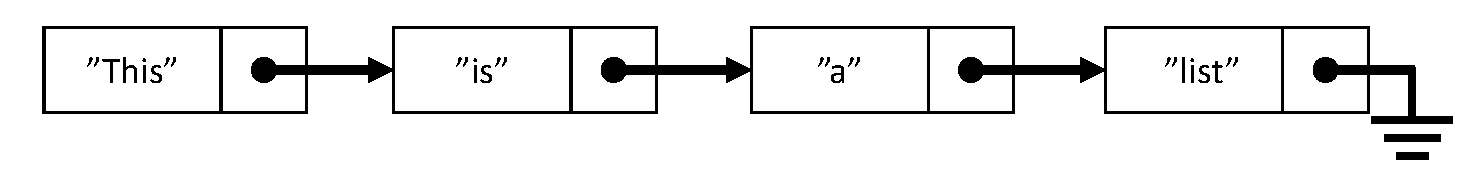
\includegraphics[width=0.75\textwidth]{linkedList}
  \caption{A list is a linked list: Here is illustrated the linked list of \mbox{\lstinline!["This"; "is"; "a"; "list"]!}.}
  \label{fig:linkedList}
\end{figure}
As a consequence, indexing element $i$ has \idx{computational complexity} $\mathcal{O}(i)$. The computational complexity of an operation is a description of how long a computation will take without considering the hardware it is performed on. The notation is sometimes called \idx{Big-O} notation or \idx{Landau notation}. In the present case, the complexity is $\mathcal{O}(i)$, which means that the complexity is linear in $i$ and indexing element $i+1$ takes $1$ unit longer than indexing element $i$ when $i$ is very large. The size of the unit is on purpose unspecified and depends on implementation and hardware details. Nevertheless, Big-O notation is a useful tool for reasoning about the efficiency of an operation. F\# has access to the list's elements only by traversing the list from its beginning. I.e., to obtain the value of element $i$, F\# starts with element 0, follows the link to element 1 and so on, until element $i$ is reached. To reach element $i+1$ instead, we would need to follow 1 more link, and assuming that following a single link takes some constant amount of time we find that the computational complexity is $\mathcal{O}(i)$.
Compared to arrays, to be discussed below, this is slow, which is why \advice{indexing lists should be avoided.}

Notice especially that lists are zero-indexed, and thus, the last element in a list \lstinline{lst} is \lstinline{lst.Length -1}. This is a very common source of error! Therefore, indexing in lists using \idx{for}-loops is supported using a special notation with the \idx[in@\lstinline{in}]{\keyword{in}} keyword,
\begin{verbatimwrite}{\ebnf/forLoopIn.ebnf}
for <*ident*> in <*list*> do <*bodyExpr*> [*done*]
\end{verbatimwrite}
\syntax{\ebnf/forLoopIn.ebnf}{For-in loop with in expression.}
In \keyword{for}-\keyword{in} loops, the loop runs through each element of the \lstinline[language=syntax]{<*list*>}, and assigns it to the identifier \lstinline[language=syntax]{<*ident*>}. This is demonstrated in \Cref{listFor}.
%
\fs{listFor}{The \keyword{for}-\keyword{in} loops are preferred over \keyword{for}-\keyword{to} loops.}
%
Using \keyword{for}-\keyword{in}-expressions remove the risk of off-by-one indexing errors, and thus, \advice{\keyword{for}-\keyword{in} is to be preferred over \keyword{for}-\keyword{to}.}

Lists support slicing identically to strings, as demonstrated in \Cref{listSlicing}.
%
\fsOutput{listSlicing}{Examples of list slicing. Compare with \Cref{stringIndexing}.}
%

Lists may be concatenated using either the \idx[{@}@{\lstinline{@}}]{\lexeme{@}}\jon{why does the at-symbol not appear in the index?} \idx[list concatenation]{concatenation} operator or the \idx[::@\lstinline{::}]{\lexeme{::}} \idx[list cons]{cons} operators. The difference is that \lexeme{@} concatenates two lists of identical types, while \lexeme{::} concatenates an element and a list of identical types.  This is demonstrated in \Cref{listCon}.
%
\fsOutput{listCon}{Examples of list concatenation.}
%
Since lists are represented as linked lists, the cons operator is very efficient and has computational complexity $\mathcal{O}(1)$, while concatenation has computational complexity $\mathcal{O}(n)$, where $n$ is the length of the first list.


It is possible to make multidimensional lists as lists of lists, as shown in \Cref{listMultidimensional}. 
%
\fs{listMultidimensional}{A ragged multidimensional list, built as lists of lists, and its indexing.}
%
The example shows a \idx{ragged multidimensional list}, since each row has a different number of elements. This is also illustrated in \Cref{fig:raggedLinkedList}.
\begin{figure}
  \centering
  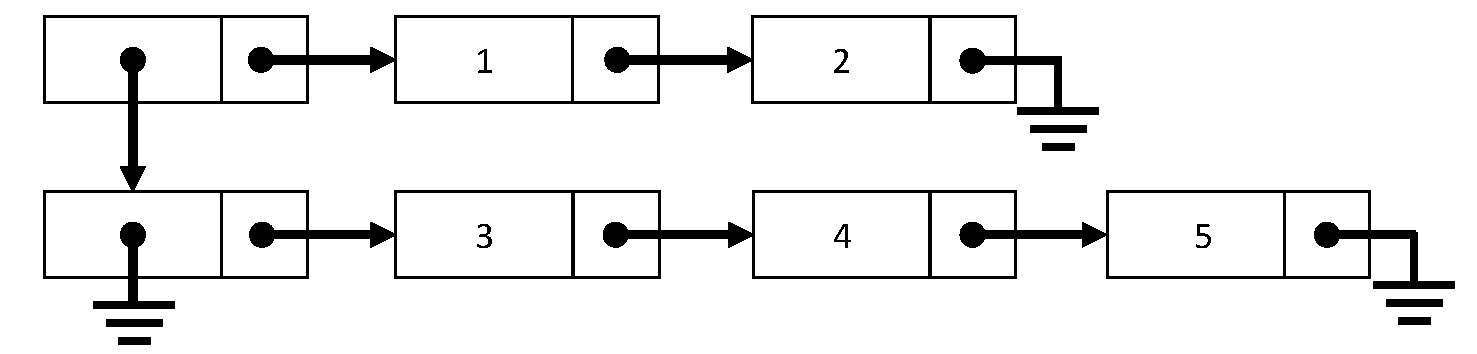
\includegraphics[width=0.75\textwidth]{raggedLinkedList}
  \caption{A list is a ragged linked list: Here is illustrated the linked list of \mbox{\lstinline![[1;2];[3;4;5]]!}.}
  \label{fig:raggedLinkedList}
\end{figure}

 The indexing of a particular element is slow due to the linked list implementation of lists, which is why arrays are often preferred for two- and higher-dimensional data structures, see \Cref{sec:arrays}.
 \clearpage
 
\section{List Properties}
Lists support a number of properties, some of which are listed below.
\begin{description}
\item[\texttt{Head}:] Returns the first element of a list.
  \fsOutputNF{listHeadProp}{\lstinline{Head}}~\\
  \idxss{Head@\lstinline{Head}}
\item[\texttt{IsEmpty}:] Returns true if the list is empty.
  \fsOutputNF{listIsEmptyProp}{\lstinline{IsEmpty}}~\\
  \idxss{IsEmpty@\lstinline{IsEmpty}}
\item[\texttt{Length}:] Returns the number of elements in the list.
  \fsOutputNF{listLengthProp}{\lstinline{Length}}~\\
  \idxss{Length@\lstinline{Length}}
\item[\texttt{Tail}:] Returns the list, except for its first element.
  \fsOutputNF{listTailProp}{\lstinline{Tail}}~\\
  \idxss{Head@\lstinline{Tail}}
\end{description}

\section{The List Module}
The built-in \lstinline{List} module contains a wealth of functions for lists, some of which are
%including \lstinline!List.length!, \lstinline!List.isEmpty!, \lstinline!List.item!, \lstinline!List.head!, \lstinline!List.tail! for working with list. 
%The basic properties and members of lists are 
briefly summarized below:
%\Cref{tab:list,tab:listCont}.\idxss{Length}\idxss{List.Empty}\idxss{IsEmpty}\idxss{Item}\idxss{Head}\idxss{Tail}\idxss{Cons}
\begin{description}
\item[\texttt{List.collect}:] \lstinline{f:('T -> 'U list) -> lst:'T list -> 'U list}.~\\
  Applies \lstinline{f} to each element in \lstinline{lst} and return a concatenated list of the results.
  \fsOutputNF{listCollect}{\lstinline{List.collect}}\idxss{List.collect@\lstinline{List.collect}}
\item[\texttt{List.contains}:] \lstinline{elm:'T -> lst:'T list -> bool}.~\\
  Returns true or false depending on whether or not \lstinline{elm} is contained in \lstinline{lst}.
  \fsOutputNF{listContains}{\lstinline{List.contains}}\idxss{List.contains@\lstinline{List.contains}}
  % \item[\texttt{List.empty}:]  \lstinline{'T list}.~\\
  %An empty list of inferred type.
%  \fsOutputNF{listEmpty}{\lstinline{List.empty}}\idxss{List.empty@\lstinline{List.empty}}
% \item[\texttt{List.exists}:] \lstinline{('T -> bool) -> 'T list -> bool}. Returns true or false depending on whether any element is true for a given function.
%   \fsOutputNF{listExists}{\lstinline{List.exists}}\idxss{List.exists@\lstinline{List.exists}}
\item[\texttt{List.filter}:] \lstinline{f:('T -> bool) -> lst:'T list -> 'T list}.~\\
  Returns a new list with all the elements of \lstinline{lst} for which \lstinline{f} evaluates to true.
  \fsOutputNF{listFilter}{\lstinline{List.filter}}\idxss{List.filter@\lstinline{List.filter}}
\item[\texttt{List.find}:] \lstinline{f:('T -> bool) -> lst:'T list -> 'T}.~\\
  Returns the first element of \lstinline{lst} for which \lstinline{f} is true.
  \fsOutputNF{listFind}{\lstinline{List.find}}\idxss{List.find@\lstinline{List.find}}
\item[\texttt{List.findIndex}:] \lstinline{f:('T -> bool) -> lst:'T list -> int}.~\\
  Returns the index of the first element of \lstinline{lst} for which \lstinline{f} is true.
  \fsOutputNF{listFindIndex}{\lstinline{List.findIndex}}\idxss{List.findIndex@\lstinline{List.findIndex}}
\item[\texttt{List.fold}:] \lstinline{f:('S -> 'T -> 'S) -> elm:'S -> lst:'T list -> 'S}.~\\
  Updates an accumulator iteratively by applying \lstinline{f} to each element in \lstinline{lst}. The initial value of the accumulator is \lstinline{elm}. For example, when \lstinline{lst} consists of \lstinline{n+1} elements
  % \lstinline{[x}$_0$\lstinline{; x}$_1$\lstinline{; x}$_2$\lstinline{;} $\ldots$\lstinline{; x}$_n$\lstinline{]}, a supplied function \lstinline{f}, and an initial value for the accumulator \lstinline{elm},
  \lstinline{List.fold} calculates:
  \begin{quote}
    \lstinline{f (}$\ldots$ \lstinline{(f (f elm lst.[0]) lst.[1])} $\ldots$\lstinline{) lst.[n]}.
  \end{quote}
  \fsOutputNF{listFold}{\lstinline{List.fold}}\idxss{List.fold@\lstinline{List.fold}}
\item[\texttt{List.foldBack}:] \lstinline{f:('T -> 'S -> 'S) -> lst:'T list -> elm:'S -> 'S}.~\\
  Updates an accumulator iteratively backwards by applying \lstinline{f} to each element in \lstinline{lst}. The initial value of the accumulator is \lstinline{elm}. For exampel, when \lstinline{lst} consists of \lstinline{n+1} elements
  %function to each element in a list, e.g., for a list consisting of $x_0, x_1, x_2, \ldots, x_n$, a supplied function $f$, and an initial value for the accumulator $s$, \lstinline{List.foldBack} calculates $f(x_0, f(x_1, f(x_2, \ldots, f(x_n, s))))$.
  \lstinline{List.foldBack} calculates:
  \begin{quote}
    \lstinline{f lst.[0] (f lst.[1]} ($\ldots$\lstinline{(f lst.[n] elm)} $\ldots$\lstinline{))}.
  \end{quote}
  \fsOutputNF{listFoldBack}{\lstinline{List.foldBack}}\idxss{List.foldBack@\lstinline{List.foldBack}}
\item[\texttt{List.forall}:] \lstinline{f:('T -> bool) -> lst:'T list -> bool}.~\\
  Returns true if all elements in \lstinline{lst} are true when \lstinline{f} is applied to them.
  \fsOutputNF{listForall}{\lstinline{List.forall}}\idxss{List.forall@\lstinline{List.forall}}
\item[\texttt{List.head}:] \lstinline{lst:'T list -> int}.~\\
  Returns the first element in \lstinline{lst}. An exception is raised if \lstinline{lst} is empty. See \Cref{sec:exceptions} for more on exceptions.
  \fsOutputNF{listHeadAlt}{\lstinline{List.head}}\idxss{List.head@\lstinline{List.head}}
\item[\texttt{List.init}:] \lstinline{m:int -> f:(int -> 'T) -> 'T list}.~\\
  Create a list with \lstinline{m} elements and whose value is the result of applying \lstinline{f} to the index of the element.
  \fsOutputNF{listInit}{\lstinline{List.init}}\idxss{List.init@\lstinline{List.init}}
\item[\texttt{List.isEmpty}:]  \lstinline{lst:'T list -> bool}.~\\
  Returns true if \lstinline{lst} is empty.
  \fsOutputNF{listIsEmptyAlt}{\lstinline{List.isEmpty}}\idxss{List.isEmpty@\lstinline{List.isEmpty}}
  % \item[\texttt{List.item}:]  \lstinline{'T list -> int}.~\\
  %Retrieves an element of a list by its index.
%   \fsOutputNF{listItemAlt}{\lstinline{List.item}}\idxss{List.item@\lstinline{List.item}}
\item[\texttt{List.iter}:] \lstinline{f:('T -> unit) -> lst:'T list -> unit}.~\\
  Applies \lstinline{f} to every element in \lstinline{lst}.
  \fsOutputNF{listIter}{\lstinline{List.iter}}\idxss{List.iter@\lstinline{List.iter}}
% \item[\texttt{List.Length}:]  \lstinline{'T list -> int}. Returns the number of elements in a list.
%   \fsOutputNF{listLengthAlt}{\lstinline{List.Length}}\idxss{List.Length@\lstinline{List.Length}}
\item[\texttt{List.map}:] \lstinline{f:('T -> 'U) -> lst:'T list -> 'U list}.~\\
  Returns a list as a concatenation of applying \lstinline{f} to every element of \lstinline{lst}.
  \fsOutputNF{listMap}{\lstinline{List.map}}\idxss{List.map@\lstinline{List.map}}
\item[\texttt{List.ofArray}:] \lstinline{arr:'T [] -> 'T list}.~\\
  Returns a list whose elements are the same as \lstinline{arr}. See \Cref{sec:arrays} for more on arrays.
  \fsOutputNF{listOfArray}{\lstinline{List.ofArray}}\idxss{List.ofArray@\lstinline{List.ofArray}}
\item[\texttt{List.rev}:] \lstinline{lst:'T list -> 'T list}.~\\
  Returns a new list with the same elements as in \lstinline{lst} but in reversed order.
  \fsOutputNF{listRev}{\lstinline{List.rev}}\idxss{List.rev@\lstinline{List.rev}}
\item[\texttt{List.sort}:] \lstinline{lst:'T list -> 'T list}.~\\
  Returns a new list with the same elements as in \lstinline{lst} but where the elements are sorted.
  \fsOutputNF{listSort}{\lstinline{List.sort}}\idxss{List.sort@\lstinline{List.sort}}
\item[\texttt{List.tail}:]  \lstinline{'T list -> 'T list}.~\\
  Returns a new list identical to \lstinline{lst} but without its first element. An Exception is raised if \lstinline{lst} is empty.  See \Cref{sec:exceptions} for more on exceptions.
  \fsOutputNF{listTailAlt}{\lstinline{List.tail}}\idxss{List.tail@\lstinline{List.tail}}
\item[\texttt{List.toArray}:] \lstinline{lst:'T list -> 'T []}.~\\
  Returns an array whose elements are the same as \lstinline{lst}.  See \Cref{sec:arrays} for more on arrays.
  \fsOutputNF{listToArray}{\lstinline{List.toArray}}\idxss{List.toArray@\lstinline{List.toArray}}
\item[\texttt{List.unzip}:] \lstinline{lst:('T1 * 'T2) list -> 'T1 list * 'T2 list}.~\\
  Returns a pair of lists of all the first elements and all the second elements of \lstinline{lst}, respectively.
  \fsOutputNF{listUnzip}{\lstinline{List.unzip}}\idxss{List.unzip@\lstinline{List.unzip}}
\item[\texttt{List.zip}:] \lstinline{lst1:'T1 list -> lst2:'T2 list -> ('T1 * 'T2) list}.~\\
  Returns a list of pairs, where elements in \lstinline{lst1} and \lstinline{lst2} are iteratively paired.
  \fsOutputNF{listZip}{\lstinline{List.zip}}\idxss{List.zip@\lstinline{List.zip}}
\end{description}

\section{Key concepts and terms in this chapter}
Summary text about the key concepts from this chapter
\begin{itemize}
\item \ldots
\end{itemize}
\end{document}
